\documentclass{article}\usepackage[]{graphicx}\usepackage[]{color}
%% maxwidth is the original width if it is less than linewidth
%% otherwise use linewidth (to make sure the graphics do not exceed the margin)
\makeatletter
\def\maxwidth{ %
  \ifdim\Gin@nat@width>\linewidth
    \linewidth
  \else
    \Gin@nat@width
  \fi
}
\makeatother

\definecolor{fgcolor}{rgb}{0.345, 0.345, 0.345}
\newcommand{\hlnum}[1]{\textcolor[rgb]{0.686,0.059,0.569}{#1}}%
\newcommand{\hlstr}[1]{\textcolor[rgb]{0.192,0.494,0.8}{#1}}%
\newcommand{\hlcom}[1]{\textcolor[rgb]{0.678,0.584,0.686}{\textit{#1}}}%
\newcommand{\hlopt}[1]{\textcolor[rgb]{0,0,0}{#1}}%
\newcommand{\hlstd}[1]{\textcolor[rgb]{0.345,0.345,0.345}{#1}}%
\newcommand{\hlkwa}[1]{\textcolor[rgb]{0.161,0.373,0.58}{\textbf{#1}}}%
\newcommand{\hlkwb}[1]{\textcolor[rgb]{0.69,0.353,0.396}{#1}}%
\newcommand{\hlkwc}[1]{\textcolor[rgb]{0.333,0.667,0.333}{#1}}%
\newcommand{\hlkwd}[1]{\textcolor[rgb]{0.737,0.353,0.396}{\textbf{#1}}}%
\let\hlipl\hlkwb

\usepackage{framed}
\makeatletter
\newenvironment{kframe}{%
 \def\at@end@of@kframe{}%
 \ifinner\ifhmode%
  \def\at@end@of@kframe{\end{minipage}}%
  \begin{minipage}{\columnwidth}%
 \fi\fi%
 \def\FrameCommand##1{\hskip\@totalleftmargin \hskip-\fboxsep
 \colorbox{shadecolor}{##1}\hskip-\fboxsep
     % There is no \\@totalrightmargin, so:
     \hskip-\linewidth \hskip-\@totalleftmargin \hskip\columnwidth}%
 \MakeFramed {\advance\hsize-\width
   \@totalleftmargin\z@ \linewidth\hsize
   \@setminipage}}%
 {\par\unskip\endMakeFramed%
 \at@end@of@kframe}
\makeatother

\definecolor{shadecolor}{rgb}{.97, .97, .97}
\definecolor{messagecolor}{rgb}{0, 0, 0}
\definecolor{warningcolor}{rgb}{1, 0, 1}
\definecolor{errorcolor}{rgb}{1, 0, 0}
\newenvironment{knitrout}{}{} % an empty environment to be redefined in TeX

\usepackage{alltt}
\title{Problem Set 7}
\author{Cameron Adams}


\usepackage{float, hyperref}
\usepackage[margin = 1in]{geometry}
\usepackage{graphicx}
\usepackage{sectsty}
\usepackage{hyperref}
\usepackage{amsmath}
\IfFileExists{upquote.sty}{\usepackage{upquote}}{}
\begin{document}
%\SweaveOpts{concordance=TRUE}

\maketitle





%Q1
\section{Suppose I have a statistical method that estimates a regression ...}

%You can compare the standard error, $SE(\hat{\beta})_{1,...,m}$, from the distribution of estimate coefficients, $\hat{\beta}_{1,...,m}$. Compare these estimated SE, $\hat{\beta}_{1,...,m}$ , to the SE of the coefficient, $\widehat{SE}(\hat{\beta})$.


You can compare the standard errors estimated from simulation study, $\hat{SE}_i(\hat{\beta})_i$, to the standard error of the estimated coefficients $SE(\hat{\beta}_i)$ or to the mean of the estimated standard errors, $mean(\hat{SE}(\hat{\beta}_i))$.


\section{Show that $||A||_2$ is the largest of the absolute values of the eigenvalues of A for symmetric A. To do so, find the following quantity ...}

First we assume that A is symmetric, with $A = \Gamma \Lambda \Gamma^{-1}$, where, $\Lambda$ is a diagonal matrix of eigenvalues and $\Lambda$ are the eigenvectors.

$$\begin{aligned}
||A||_2 &= \sup_{z:||z||_2} \sqrt{(Az)^\top Az} \\
&= \sqrt{z^\top A^\top Az} \\
&= \sqrt{z^\top (\Gamma \Lambda \Gamma^{-1})^\top (\Gamma \Lambda \Gamma)z} \\
&= \sqrt{z^\top (\Gamma^{-1})^\top \Lambda \Gamma^\top \Gamma \Lambda \Gamma^{-1}z} \\
&= \sqrt{(\Gamma^{-1} z)^\top \Lambda^2 (\Gamma^{-1} z)} \\
\text{where } y &= \Gamma^\top z, \text{and if } ||z||_2 = 1 \text{ then } ||y||_2 = 1 \\
&= y^\top \Lambda^2 y \\
&= \sum_{i=1}^n \sqrt{ \sum_{i=1}^n \lambda_i y_i^2} \\
\text{maximized when} &\sqrt{ \sum_{i=1}^n \lambda_i y_i^2} = \sqrt{max(|\lambda_i|)} \\
\end{aligned}$$

We can use the hint $\Gamma^\top z = y$ because $\Gamma$ is orthogonal columns (SVD). Therefore, if $||z||_2=1$ then it follows that $||y||_2 =1$. The norms of the columns of $\Gamma$ are 1 by SVD. Therefore, the linear map of $\Gamma$ applied to unit norm vector will give a unit norm vector output. When we get to the sum, we know that $\sum y_i = 1$. From there we can substitute the $\sum$ into the equation, and we know that this value is maximized when we have the largest singular/eigen value, which should be the first one.

%3
\section{Some practice with matrix manipulations.}

\subsection{}

X is a matrix with n x p dimensions, with n $>$ p. $X^\top X = M$, where $M$ is a matrix of dimension p x p and $X X^\top= M$ and $M$ is a matrix with dimensions n x n. Therefore, the eigen decomposition of $X^\top X$, by definition of SVD:

$$\begin{aligned}
\text{by definition, SVD of } X = UDV^\top &\\
\text{therefore, } &\\
X^\top X  &= (UDV^\top)^\top (UDV^\top) \\
&= (VD^\top U^\top UDV^\top \\ 
&= V D^\top D V^\top \\
&= V D^2 V^\top \\
\end{aligned}$$

And for $X X^\top = M$, we see something similar


$$\begin{aligned}
\text{by definition, SVD of } X = UDV^\top &\\
\text{therefore, } & \\
X^\top X  &= (UDV^\top)(UDV^\top)^\top  \\
& = U D V^\top V D^\top U^\top \\
& = U D^2 U^\top  \\
\end{aligned}$$

Therefore, we see that the left and right singular vectors of $X$ are the eigenvalues for $XX^\top$ and $X^\top X$, respectively.

To show that $X^\top X$ is p.s.d., we need  the eigenvalues of $X^\top X$ to be positive and that $X^\top X$ is symmetric. From above, we see that eigen-decomposition of  $X^\top X = V D^2 V^\top$. The eigenvalues are $D^2$, and $D^2>0$. $X^\top X$ will be a square matrix with dimensions p x p, and is symmetric and therefore will be positive definite.


\subsection{}
If we know that $\lambda$ is a number that is an eigenvalue of $\Sigma$ and $v$ is a non-zero vector that is an eigenvector of $\Sigma$, there, $\Sigma v = \lambda v$. So, if we want an eigenvalue for $Z = \Sigma + c I$, we can substitute $Z$ for $\Sigma$.

$$\begin{aligned}
Z v &= \lambda v \\
(\Sigma + c I) v &= \lambda v \\
(\Sigma + c I) &= \lambda \\
\end{aligned}$$

\section{}



\subsection{}

First I would simplify the expression by inverting $AC^{-1}A^\top)^{-1}$.

$$\begin{aligned}
\beta &= C^{-1} d +C^{-1}A^\top (AC^{-1}A^\top)^{-1} (-AC^{-1}d + b) \\
&= C^{-1} d + C^-1 A^\top (A^\top)^{-1}C A^{-1} (-AC^{-1}d + b) \\
&= C^{-1} d + A^{-1}  (-AC^{-1}d + b) \\
&= C^{-1} d + A^{1} A C^{-1}d + A^{-1} b \\
&= C^{-1} d - C^{-1} d + A^{-1}b \\
&=  A^{-1}b
\end{aligned}$$

In the above simplification, we are assuming that $A$ is invertable. However, if we can't assume $A$ is invertable, then we can use eigen decomposition to remove the need for taking the inverse of $E^{-1} =(AC^{-1}A^\top)^{-1}$.

$$\begin{aligned}
\beta &= C^{-1} d +C^{-1}A^\top (AC^{-1}A^\top)^{-1} (-AC^{-1}d + b) \\
&= C^{-1} d +C^{-1}A^\top (eigen(AC^{-1}A^\top))^{-1} (-AC^{-1}d + b) \\
&= C^{-1} d +C^{-1}A^\top (\Gamma \Lambda \Gamma^\top)^{-1} (-AC^{-1}d + b) \\
&= C^{-1} d +C^{-1}A^\top (\Gamma^\top)^{-1} \Lambda^{-1} \Gamma^{-1} (-AC^{-1}d + b) \\
&= C^{-1} d +C^{-1}A^\top \Gamma \Lambda^{-1} \Gamma^\top (-AC^{-1}d + b) \\
\end{aligned}$$

If we assume, that the eigenvalues in $\Lambda > 0$, then we can use backsolve Cholesky and backsolves for $C^{-1} d$ and $C^{-1}A$ expressions. We would then want to solve this system from right to left.


\subsection{}

We could write up three functions and one expression to solve this matrix: 

\begin{enumerate}
    \item q3.fun.solve(): The original way using $solve()$, which is the bad way
    \item q3.fun.fast(): Use cholesky decomposition and some $backsolve()$'s to reduce the number of $solve()$'s
    \item q3.fun.eigen(): Use eigen decomposition, cholesky decomposition, and $backsolve$'s to remove all $solve()$'s [MY ANSWER]
    \item Simply $\beta = A^{-1}b$
\end{enumerate}

The third function is my answer and probably the most correct. The fourth is the most fun.
\begin{knitrout}
\definecolor{shadecolor}{rgb}{0.969, 0.969, 0.969}\color{fgcolor}\begin{kframe}
\begin{alltt}
\hlkwd{rm}\hlstd{(}\hlkwc{list}\hlstd{=}\hlkwd{ls}\hlstd{())}
\hlkwd{gc}\hlstd{()}
\hlkwd{require}\hlstd{(MASS)}

\hlstd{m} \hlkwb{=} \hlnum{50}
\hlstd{p} \hlkwb{=} \hlnum{20}
\hlstd{n} \hlkwb{=} \hlnum{100}

\hlstd{X} \hlkwb{=} \hlkwd{matrix}\hlstd{(}\hlkwd{rnorm}\hlstd{(n}\hlopt{*}\hlstd{p),} \hlkwc{ncol} \hlstd{= p)}
\hlstd{d} \hlkwb{=} \hlkwd{matrix}\hlstd{(}\hlkwd{rnorm}\hlstd{(p),} \hlkwc{ncol} \hlstd{=} \hlnum{1}\hlstd{)}
\hlstd{A} \hlkwb{=} \hlkwd{matrix}\hlstd{(}\hlkwd{rnorm}\hlstd{(m}\hlopt{*}\hlstd{p),} \hlkwc{ncol} \hlstd{= p)}
\hlstd{b} \hlkwb{=} \hlkwd{matrix}\hlstd{(}\hlkwd{rnorm}\hlstd{(m),} \hlkwc{ncol} \hlstd{=} \hlnum{1}\hlstd{)}

\hlcom{#1}
\hlstd{q3.fun.solve} \hlkwb{<-} \hlkwa{function}\hlstd{(}\hlkwc{X}\hlstd{,} \hlkwc{d}\hlstd{,} \hlkwc{A}\hlstd{,} \hlkwc{b}\hlstd{) \{}

    \hlcom{#get C}
    \hlstd{C} \hlkwb{=} \hlkwd{crossprod}\hlstd{(X)} \hlcom{#symmetric t(X) %*% X}

    \hlcom{#caculate parts of expression     }
    \hlstd{first}  \hlkwb{=} \hlkwd{solve}\hlstd{(C)} \hlopt \hlstd{d}
    \hlstd{second} \hlkwb{=} \hlkwd{solve}\hlstd{(C)} \hlopt \hlkwd{t}\hlstd{(A)}
    \hlstd{third}  \hlkwb{=} \hlkwd{ginv}\hlstd{(A} \hlopt \hlkwd{solve}\hlstd{(C)} \hlopt \hlkwd{t}\hlstd{(A),} \hlkwc{tol} \hlstd{=} \hlnum{1} \hlopt{*} \hlstd{(.Machine}\hlopt{$}\hlstd{double.eps))}
    \hlstd{fourth} \hlkwb{=} \hlopt{-}\hlstd{A} \hlopt \hlkwd{solve}\hlstd{(C)} \hlopt \hlstd{d} \hlopt{+} \hlstd{b}

    \hlcom{#solve from right ot left}
    \hlstd{first} \hlopt{+} \hlstd{(second} \hlopt \hlstd{(third} \hlopt \hlstd{fourth))}
\hlstd{\}}

\hlcom{#2}
\hlstd{q3.fun.fast} \hlkwb{<-} \hlkwa{function}\hlstd{(}\hlkwc{X}\hlstd{,} \hlkwc{d}\hlstd{,} \hlkwc{A}\hlstd{,} \hlkwc{b}\hlstd{) \{}

    \hlcom{#Chol decomposition for C = X^tX}
    \hlstd{U} \hlkwb{<-} \hlkwd{chol}\hlstd{(}\hlkwd{crossprod}\hlstd{(X),} \hlkwc{pivot} \hlstd{= T)} \hlcom{# U is upper-triangular }

    \hlcom{#caculate parts of expression    }
    \hlstd{first}  \hlkwb{=} \hlkwd{backsolve}\hlstd{(U, d)}
    \hlstd{second} \hlkwb{=} \hlkwd{backsolve}\hlstd{(U,} \hlkwd{t}\hlstd{(A))}
    \hlstd{third}  \hlkwb{=} \hlkwd{ginv}\hlstd{(A} \hlopt \hlkwd{backsolve}\hlstd{(U,} \hlkwd{t}\hlstd{(A)),} \hlkwc{tol} \hlstd{=} \hlnum{1} \hlopt{*} \hlstd{(.Machine}\hlopt{$}\hlstd{double.eps))}
    \hlstd{fourth} \hlkwb{=} \hlopt{-}\hlstd{A} \hlopt \hlkwd{backsolve}\hlstd{(U, d)} \hlopt{+} \hlstd{b}

    \hlcom{#solve from right ot left}
    \hlstd{first} \hlopt{+} \hlstd{(second} \hlopt \hlstd{(third} \hlopt \hlstd{fourth))}
\hlstd{\}}

\hlcom{#3}
\hlstd{q3.fun.eigen} \hlkwb{<-} \hlkwa{function}\hlstd{(}\hlkwc{X}\hlstd{,} \hlkwc{d}\hlstd{,} \hlkwc{A}\hlstd{,} \hlkwc{b}\hlstd{) \{}

    \hlcom{#Chol decomposition for C = X^tX}
    \hlstd{U} \hlkwb{<-} \hlkwd{chol}\hlstd{(}\hlkwd{crossprod}\hlstd{(X),} \hlkwc{pivot} \hlstd{= T)} \hlcom{# U is upper-triangular }

    \hlcom{#calculate parts of expression    }
    \hlstd{first}  \hlkwb{=} \hlkwd{backsolve}\hlstd{(U, d)}
    \hlstd{second} \hlkwb{=} \hlkwd{backsolve}\hlstd{(U,} \hlkwd{t}\hlstd{(A))}
    \hlstd{E}      \hlkwb{=} \hlstd{A} \hlopt \hlkwd{ginv}\hlstd{(C)} \hlopt \hlkwd{t}\hlstd{(A)}
    \hlstd{E_eigen}\hlkwb{=} \hlkwd{eigen}\hlstd{(E)}
    \hlstd{third} \hlkwb{=} \hlstd{E_eigen}\hlopt{$}\hlstd{vectors} \hlopt \hlkwd{diag}\hlstd{(}\hlnum{1}\hlopt{/}\hlstd{E_eigen}\hlopt{$}\hlstd{values)} \hlopt \hlstd{E_eigen}\hlopt{$}\hlstd{vectors}
    \hlstd{fourth} \hlkwb{=} \hlopt{-}\hlstd{A} \hlopt \hlkwd{backsolve}\hlstd{(U, d)} \hlopt{+} \hlstd{b}

    \hlcom{#solve from right ot left}
    \hlstd{first} \hlopt{+} \hlstd{(second} \hlopt \hlstd{(third} \hlopt \hlstd{fourth))}
\hlstd{\}}

\hlcom{#4}
\hlstd{beta} \hlkwb{<-} \hlkwd{solve}\hlstd{(A)} \hlopt \hlstd{b}
\end{alltt}
\end{kframe}
\end{knitrout}

%question 5
\section{}


\subsection{}
We cannot compute this matrix directly, even if we use matrix decomposition simply because the resulting matrices would be very very large. Memory space would be the biggest concern, but it would also be computational difficult to perform computations with matrices that are millions x millions in size without first reducing them, or performing sparse matrix operations.

\subsection{}

We can rewrite the equations, by expanding $X$ an $X^\top$ in the equation for $\hat{\beta}$. From there we can simplify and perform matrix operations and will result in matrices of manageable size. See below.


$$\begin{aligned}
\text{If, }& \\
\hat{X} &= Z(Z^\top Z)^{-1} Z^\top X \text{ and }\\
\hat{X}^\top &= X^\top Z ((Z^\top Z)^{-1})^\top Z^\top \text{ then,}\\
\beta &= (\hat{X}^\top \hat{X})^{-1} \hat{X}^\top y \\
\beta &= [(X^\top Z ((Z^\top Z)^{-1})^\top Z^\top) (Z (Z^\top Z)^{-1} Z^\top X)]^{-1} (X^\top Z ((Z^\top Z)^{-1})^\top Z^\top) y \\  
\beta &= (X^\top Z ((Z^\top Z)^{-1})^\top X)^{-1} X^\top Z ((Z^\top Z)^{-1})^\top Z^\top y \\
\end{aligned}$$

Now, in this form, we have a series of matrix operations and will HUGELY reduce the size of the matrices used for calculation of $\beta$

$$\begin{aligned}
A &= X^\top Z = Z^\top X : \text{(630x60M)(60Mx1)=630x1}\\
B &= ((Z^\top Z)^{-1})^\top : \text{(630x60M)(60Mx630)=630x630}\\
C &= Z^\top y :  \text{(630x60M)(60Mx630)=630x630} \\
\end{aligned}$$

From here, we could plug in these much smaller matrices, $A, B, C$, into the expanded equation from above:

$$\begin{aligned}
\beta &= (X^\top Z ((Z^\top Z)^{-1})^\top X)^{-1} X^\top Z ((Z^\top Z)^{-1})^\top Z^\top y \\
\end{aligned}$$

This should be fairly easy to compute even for a regular computer. If memory were of particular concern, we could also remove the original matrices, $Z, X, y$ from memory after we compute, $A, B, C$.


%6
\section{}

\begin{knitrout}
\definecolor{shadecolor}{rgb}{0.969, 0.969, 0.969}\color{fgcolor}\begin{kframe}
\begin{alltt}
\hlkwd{rm}\hlstd{(}\hlkwc{list}\hlstd{=}\hlkwd{ls}\hlstd{())}

\hlcom{#generate z matrix}
\hlstd{n}\hlkwb{=}\hlnum{100}
\hlstd{z} \hlkwb{=} \hlkwd{matrix}\hlstd{(}\hlkwd{rnorm}\hlstd{(n} \hlopt{*} \hlstd{n),} \hlkwc{ncol} \hlstd{= n)}

\hlcom{#eigen decomp}
\hlstd{z_eigen} \hlkwb{=} \hlkwd{eigen}\hlstd{(} \hlkwd{crossprod}\hlstd{(z) )}
\hlstd{Gamma}  \hlkwb{<-} \hlstd{z_eigen}\hlopt{$}\hlstd{vectors} \hlcom{#Lambda}

\hlcom{#generate eigenvalues}
\hlstd{Lambda} \hlkwb{<-} \hlkwd{sapply}\hlstd{(}\hlkwd{seq}\hlstd{(}\hlopt{-}\hlnum{1}\hlstd{,} \hlnum{32}\hlstd{,} \hlnum{2}\hlstd{),} \hlkwa{function}\hlstd{(}\hlkwc{x}\hlstd{)}
    \hlkwd{seq}\hlstd{(}\hlnum{0.1}\hlstd{,} \hlnum{0.01}\hlstd{,} \hlkwc{length.out} \hlstd{= n)} \hlopt{*}
    \hlnum{10}\hlopt{^}\hlkwd{floor}\hlstd{(}\hlkwd{seq}\hlstd{(x,} \hlopt{-}\hlnum{1}\hlstd{,} \hlkwc{length.out} \hlstd{= n)))}

\hlcom{#add text eigen values of all the same number}
\hlstd{Lambda} \hlkwb{<-} \hlkwd{cbind}\hlstd{(}\hlkwd{rep}\hlstd{(}\hlnum{0.01}\hlstd{, n),} \hlkwd{rep}\hlstd{(}\hlnum{5}\hlstd{),} \hlkwd{rep}\hlstd{(}\hlnum{11}\hlstd{), Lambda)}
\hlkwd{head}\hlstd{(Lambda)}
\end{alltt}
\begin{verbatim}
##      [,1] [,2] [,3]        [,4]       [,5]       [,6]       [,7]
## [1,] 0.01    5   11 0.010000000 1.00000000 100.000000 10000.0000
## [2,] 0.01    5   11 0.009909091 0.09909091   9.909091   990.9091
## [3,] 0.01    5   11 0.009818182 0.09818182   9.818182   981.8182
## [4,] 0.01    5   11 0.009727273 0.09727273   9.727273   972.7273
## [5,] 0.01    5   11 0.009636364 0.09636364   9.636364   963.6364
## [6,] 0.01    5   11 0.009545455 0.09545455   9.545455   954.5455
##            [,8]      [,9]       [,10]        [,11]        [,12]
## [1,] 1000000.00 100000000 10000000000 1.000000e+12 1.000000e+14
## [2,]   99090.91   9909091   990909091 9.909091e+10 9.909091e+12
## [3,]   98181.82   9818182   981818182 9.818182e+10 9.818182e+12
## [4,]   97272.73   9727273   972727273 9.727273e+10 9.727273e+12
## [5,]   96363.64   9636364   963636364 9.636364e+10 9.636364e+12
## [6,]   95454.55   9545455   954545455 9.545455e+10 9.545455e+12
##             [,13]        [,14]        [,15]        [,16]        [,17]
## [1,] 1.000000e+16 1.000000e+18 1.000000e+20 1.000000e+22 1.000000e+24
## [2,] 9.909091e+14 9.909091e+16 9.909091e+18 9.909091e+20 9.909091e+22
## [3,] 9.818182e+14 9.818182e+16 9.818182e+18 9.818182e+20 9.818182e+22
## [4,] 9.727273e+14 9.727273e+16 9.727273e+18 9.727273e+20 9.727273e+22
## [5,] 9.636364e+14 9.636364e+16 9.636364e+18 9.636364e+20 9.636364e+21
## [6,] 9.545455e+14 9.545455e+15 9.545455e+17 9.545455e+19 9.545455e+21
##             [,18]        [,19]        [,20]
## [1,] 1.000000e+26 1.000000e+28 1.000000e+30
## [2,] 9.909091e+24 9.909091e+26 9.909091e+28
## [3,] 9.818182e+24 9.818182e+26 9.818182e+28
## [4,] 9.727273e+24 9.727273e+26 9.727273e+28
## [5,] 9.636364e+23 9.636364e+25 9.636364e+27
## [6,] 9.545455e+23 9.545455e+25 9.545455e+27
\end{verbatim}
\begin{alltt}
\hlcom{#calculate condition  number}
\hlstd{cond_num} \hlkwb{<-} \hlstd{Lambda[}\hlnum{1}\hlstd{, ]} \hlopt{/} \hlstd{Lambda[}\hlnum{100}\hlstd{, ]}
\hlstd{cond_num}
\end{alltt}
\begin{verbatim}
##  [1] 1e+00 1e+00 1e+00 1e+01 1e+03 1e+05 1e+07 1e+09 1e+11 1e+13 1e+15
## [12] 1e+17 1e+19 1e+21 1e+23 1e+25 1e+27 1e+29 1e+31 1e+33
\end{verbatim}
\begin{alltt}
\hlcom{#for loop to calculate z*, lambda*, and plot(lambda, lambda*)}
\hlcom{##calculate abs difference in lambda values}
\hlkwd{par}\hlstd{(}\hlkwc{mfrow} \hlstd{=} \hlkwd{c}\hlstd{(}\hlnum{2}\hlstd{,} \hlnum{3}\hlstd{))}
\hlstd{Lambda_diff} \hlkwb{<-} \hlstd{pd_check} \hlkwb{<-} \hlkwd{c}\hlstd{()}
\hlkwa{for} \hlstd{(i} \hlkwa{in} \hlnum{1}\hlopt{:}\hlkwd{ncol}\hlstd{(Lambda)) \{}

    \hlcom{#calcuate z* using generate Lambda's and Gamma from z}
    \hlstd{z_star} \hlkwb{<-} \hlstd{Gamma} \hlopt \hlkwd{diag}\hlstd{(Lambda[ , i])} \hlopt \hlkwd{t}\hlstd{(Gamma)}

    \hlcom{#eigen decomp z* and get lambda*}
    \hlstd{Lambda_star} \hlkwb{<-} \hlkwd{eigen}\hlstd{(z_star)}\hlopt{$}\hlstd{values}

    \hlcom{#plot every fourth lambda vs lambda*}
    \hlkwa{if} \hlstd{(i} \hlopt \hlkwd{c}\hlstd{(}\hlnum{1}\hlstd{,} \hlnum{5}\hlstd{,} \hlnum{10}\hlstd{,} \hlnum{15}\hlstd{,} \hlnum{20}\hlstd{)) \{}
        \hlkwd{plot}\hlstd{(Lambda[ , i], Lambda_star,}
         \hlkwc{main} \hlstd{=} \hlkwd{paste0}\hlstd{(}\hlstr{"Cond.num: "}\hlstd{, cond_num[i],}
                       \hlstr{"\textbackslash{}nMax(Lambda):"}\hlstd{, Lambda[}\hlnum{1}\hlstd{, i]))}
        \hlkwd{abline}\hlstd{(}\hlkwc{a} \hlstd{=} \hlnum{0}\hlstd{,} \hlkwc{b} \hlstd{=} \hlnum{1}\hlstd{)}
    \hlstd{\}} \hlkwa{else} \hlstd{\{\}}

    \hlcom{#check P.D of z*}
    \hlstd{pd_check} \hlkwb{<-} \hlkwd{c}\hlstd{(pd_check,}
                  \hlkwa{if} \hlstd{(}\hlkwd{sum}\hlstd{(Lambda_star} \hlopt{<} \hlstd{.Machine}\hlopt{$}\hlstd{double.eps)} \hlopt{>} \hlnum{0}\hlstd{) \{}\hlnum{0}\hlstd{\}} \hlkwa{else} \hlstd{\{}\hlnum{1}\hlstd{\}}
    \hlstd{)}

    \hlstd{Lambda_diff} \hlkwb{<-} \hlkwd{c}\hlstd{(Lambda_diff,}
                     \hlkwd{mean}\hlstd{(}\hlkwd{abs}\hlstd{(Lambda[ , i]} \hlopt{-} \hlstd{Lambda_star)))}
\hlstd{\}}

\hlcom{#combine results}
\hlstd{result} \hlkwb{<-} \hlkwd{data.frame}\hlstd{(}\hlkwd{cbind}\hlstd{(pd_check, cond_num, Lambda[}\hlnum{1}\hlstd{, ], Lambda_diff))}
\hlkwd{colnames}\hlstd{(result)} \hlkwb{<-} \hlkwd{c}\hlstd{(}\hlstr{"Lambda*_i > 0"}\hlstd{,} \hlstr{"Condition Num."}\hlstd{,} \hlstr{"Max(Lambda)"}\hlstd{,} \hlstr{"avg(abs(Lambda - Lambda*))"}\hlstd{)}

\hlcom{#print results table}
\hlkwd{print}\hlstd{(result)}
\end{alltt}
\begin{verbatim}
##    Lambda*_i > 0 Condition Num. Max(Lambda) avg(abs(Lambda - Lambda*))
## 1              1          1e+00     1.0e-02               5.030698e-17
## 2              1          1e+00     5.0e+00               2.517986e-14
## 3              1          1e+00     1.1e+01               5.547562e-14
## 4              1          1e+01     1.0e-02               2.469813e-18
## 5              1          1e+03     1.0e+00               3.750906e-17
## 6              1          1e+05     1.0e+02               3.427263e-15
## 7              1          1e+07     1.0e+04               3.402714e-13
## 8              1          1e+09     1.0e+06               3.256274e-11
## 9              1          1e+11     1.0e+08               3.370966e-09
## 10             1          1e+13     1.0e+10               4.383111e-07
## 11             1          1e+15     1.0e+12               3.268040e-05
## 12             1          1e+17     1.0e+14               3.530970e-03
## 13             0          1e+19     1.0e+16               3.486926e-01
## 14             0          1e+21     1.0e+18               1.717030e+01
## 15             0          1e+23     1.0e+20               1.735859e+03
## 16             0          1e+25     1.0e+22               2.821720e+05
## 17             0          1e+27     1.0e+24               2.063879e+07
## 18             0          1e+29     1.0e+26               4.690645e+09
## 19             0          1e+31     1.0e+28               3.821452e+11
## 20             0          1e+33     1.0e+30               2.056957e+13
\end{verbatim}
\end{kframe}
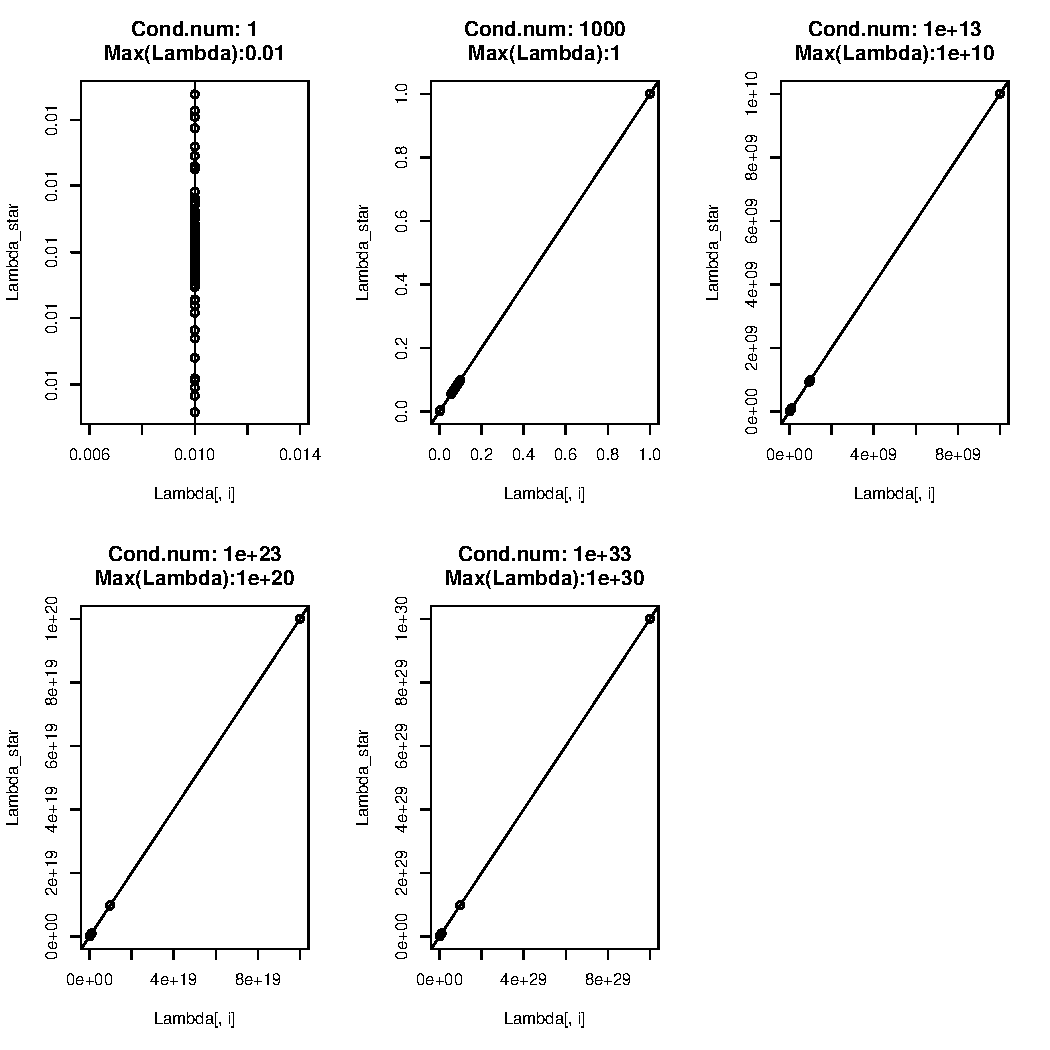
\includegraphics[width=\maxwidth]{figure/unnamed-chunk-3-1} 

\end{knitrout}

At condition number $\ge 1e17$, the z* matrix is no longer positive definite.

The error in the estimated eigenvalues doesn't begin to be noticeable until condition number $\approx 1e19$ with $max(\lambda)~\approx 1e16$. Until that point, the true and estimated eigenvalues are essentially the same with the $mean(|\Lambda - \Lambda*|)$ ranging from 1e-17 to 1e-5. Mean differenes less than machine epsilon are functionally 0.




\end{document}


